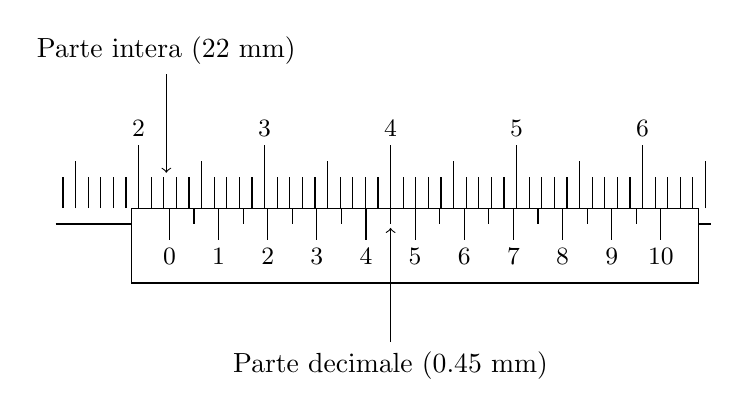
\begin{tikzpicture}%
  \node at (0, 0) {};
  \pgfmathsetmacro{\xscale}{0.16}
  \pgfmathsetmacro{\xstart}{30.}
  \pgfmathsetmacro{\y}{0.}
  {\small
  % Main scale.
  \draw[thick] (0,\y) -- (52*\xscale,\y);
  \foreach \x in {-6,-5,...,45}
  \draw[xshift=\xstart] (\x*\xscale,\y+0.2) -- (\x*\xscale,\y+0.6) {};
  \foreach \x in {-5,0,...,45}
  \draw[xshift=\xstart] (\x*\xscale,\y+0.2) -- (\x*\xscale,\y+0.8) {};
  \foreach \x in {0,10,...,45}
  \draw[xshift=\xstart] (\x*\xscale,\y+0.2) -- (\x*\xscale,\y+1.0) node[anchor=south] {\pgfmathparse{0.1*\x + 2}\pgfmathprintnumber{\pgfmathresult}};

  % Vernier scale
  \draw [fill=white,xshift=\xstart] (-3*\xscale+2.45*\xscale,\y+0.2) rectangle (42*\xscale+2.45*\xscale,\y-0.75);
  \foreach \x in {0,1,...,20}
  \draw[xshift=\xstart] (1.95*\x*\xscale+2.45*\xscale,\y+0.2) -- (1.95*\x*\xscale+2.45*\xscale,\y-0.) {};
  \foreach \x in {0,2,...,20}
  \draw[xshift=\xstart] (1.95*\x*\xscale+2.45*\xscale,\y+0.2) -- (1.95*\x*\xscale+2.45*\xscale,\y-0.2) node[anchor=north] {\pgfmathparse{0.5*\x}\pgfmathprintnumber{\pgfmathresult}};
  }

  \node[xshift=\xstart] (intera) at (2.2*\xscale,\y+2.2) {Parte intera ($22$~mm)};
  \draw[xshift=\xstart] [out=-90,in=90,-{>[scale=1.8]}] (intera) to (2.2*\xscale,\y+0.65);
  \node[xshift=\xstart] (decimale) at (1.95*9*\xscale+2.45*\xscale,\y-1.8) {Parte decimale ($0.45$~mm)};
  \draw[xshift=\xstart] [out=90,in=-90,-{>[scale=1.8]}] (decimale) to (1.95*9*\xscale+2.45*\xscale,\y-0.05);

\end{tikzpicture}
